% Fig. 2 (fig:envelope). Compile standalone with pdflatex and copy the PDF to figs/fig_envelope.pdf.
\documentclass[tikz,border=1.5pt]{standalone}
\usepackage[T1]{fontenc}
\usepackage{helvet}
\usepackage{sansmath}
\renewcommand{\familydefault}{\sfdefault}
\usetikzlibrary{arrows.meta,calc}
\definecolor{ink}{HTML}{1A1A1A}
\definecolor{mute}{HTML}{6B6B6B}
\definecolor{sClear}{HTML}{EEF7F6}\definecolor{sMild}{HTML}{D5ECEA}\definecolor{sCong}{HTML}{B9DEDB}
\begin{document}
\sansmath
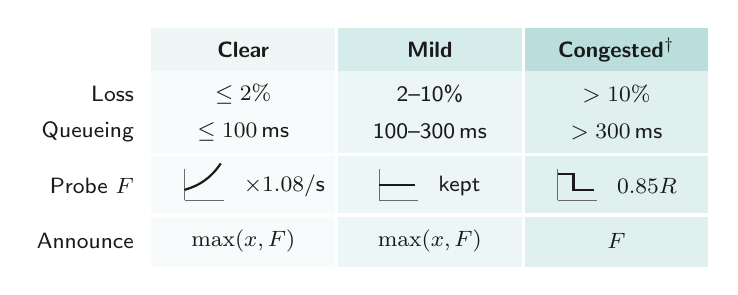
\begin{tikzpicture}[x=1cm,y=1.32cm, font=\footnotesize, text=ink]
\def\xa{1.55}\def\w{2.33}\def\g{0.04}
\pgfmathsetmacro{\xb}{\xa+\w+\g}\pgfmathsetmacro{\xc}{\xb+\w+\g}\pgfmathsetmacro{\xe}{\xc+\w}
\def\top{2.3}
\foreach \x/\c in {\xa/sClear,\xb/sMild,\xc/sCong}{\fill[\c!45] (\x,0) rectangle (\x+\w,\top);}
\foreach \x/\c/\t in {\xa/sClear/Clear,\xb/sMild/Mild,\xc/sCong/Congested$^{\dagger}$}{
  \fill[\c] (\x,\top-0.42) rectangle (\x+\w,\top);
  \node[font=\footnotesize\bfseries] at (\x+\w/2,\top-0.21) {\t};}
\def\row#1#2#3#4#5{%
  \node[anchor=east] at (\xa-0.1,#1) {#2};
  \node at (\xa+\w/2,#1) {#3};\node at (\xb+\w/2,#1) {#4};\node at (\xc+\w/2,#1) {#5};}
\row{1.66}{Loss}{$\le 2\%$}{2--10\%}{$> 10\%$}
\row{1.3}{Queueing}{$\le 100$\,ms}{100--300\,ms}{$> 300$\,ms}
\draw[white, line width=1.4pt] (\xa,1.08) -- (\xe,1.08);
\node[anchor=east] at (\xa-0.1,0.78) {Probe $F$};
\def\axes{\draw[mute, line width=0.35pt] (0,0) -- (0.5,0); \draw[mute, line width=0.35pt] (0,0) -- (0,0.3);}
\begin{scope}[shift={(\xa+0.42,0.64)}]\axes
  \draw[ink, line width=0.8pt, domain=0:0.46, samples=20] plot (\x,{0.04+0.06*exp(3.6*\x)});\end{scope}
\node[anchor=west] at (\xa+1.05,0.78) {${\times}1.08$/s};
\begin{scope}[shift={(\xb+0.52,0.64)}]\axes
  \draw[ink, line width=0.8pt] (0,0.15) -- (0.46,0.15);\end{scope}
\node[anchor=west] at (\xb+1.15,0.78) {kept};
\begin{scope}[shift={(\xc+0.42,0.64)}]\axes
  \draw[ink, line width=0.8pt] (0,0.25) -- (0.2,0.25) -- (0.2,0.1) -- (0.46,0.1);\end{scope}
\node[anchor=west] at (\xc+1.05,0.78) {$0.85R$};
\draw[white, line width=1.4pt] (\xa,0.5) -- (\xe,0.5);
\node[anchor=east] at (\xa-0.1,0.25) {Announce};
\node at (\xa+\w/2,0.25) {$\max(x, F)$};\node at (\xb+\w/2,0.25) {$\max(x, F)$};\node at (\xc+\w/2,0.25) {$F$};
\end{tikzpicture}
\end{document}
